\documentclass[a4paper, 12pt, conference]{article}

%%%%%%%%%%%%%%%%%%%%PACKAGES%%%%%%%%%%%%%%%%%%%%
\usepackage{color}  % add colors to text
\usepackage{microtype} %better letter spacing and etc
\usepackage{titling} %control the typeset of maketitle
%\usepackage[11pt]{moresize}

\usepackage{float} %allows strict placement of a float + override latex replacement -->use H

\usepackage{amsmath}  %pimp your equations
\usepackage{amssymb}  %all those extra math symbols
\usepackage{siunitx} 	% SI units

\usepackage[english]{babel}
%\usepackage[utf8]{inputenc} 
\usepackage[T1]{fontenc}  %font encoding of the input text

\usepackage{graphicx} %import graphs images and whatnot

\usepackage{caption}  %customize figure captions
\usepackage{subcaption}  %create multiple floats within a single environment giving individual captions

\usepackage{tabularx} % x designator for auto expanding width of a table column
\usepackage{tabulary} %better columns for tables: l c r j
\usepackage{booktabs} %get those pretty tables
\usepackage{booktabs} %extra commands for creating stylish tables
\usepackage{arydshln} %drawing dash lines in arrays/tabulars

\usepackage{array}  %more table handling
\usepackage{multirow} %typeset text into multiple rows
\usepackage{wrapfig} %figures with which text can flow around




%%%%%%%%%%%%%%%%%%%%PAGE FORMATTING AND WHAT NOT%%%%%%%%%%%%%%%%%%%%
\usepackage[twocolumn,hmargin=2cm,vmargin=2.5cm]{geometry}% rm if title --> full width span when 2column format

%%%%%%%%%%%%%%%%%%%%MACRO DOODLES%%%%%%%%%%%%%%%%%%%%


%%%%%%%%%%%%%%%%%%%%ABREVIATIONS AND DEFINITIONS%%%%%%%%%%%%%%%%%%%%

\def \tss {\textsuperscript}



%%%%%%%%%%%%%%%%%%%%PATHS%%%%%%%%%%%%%%%%%%%%

\graphicspath{{../rsc/}{.}{rsc/}}	



%%%%%%%%%%%%%%%%%%%%TITLE%%%%%%%%%%%%%%%%%%%%


%\author{Bian Theophile, Mathias Dankl, Mercan Samuele}
\pretitle{\begin{center}
	\vspace*{-3cm}
	
\includegraphics[scale = 0.2]{epfl_nonofficial_logo.png}\\[1cm]}
%\title{\large{\textbf{Deep Learning -- EE559 \\ Mini Neural Network Framework}}}
\posttitle{\end{center}}


%%%%%%%%%%%%%%%%%%%%DOCUMENT%%%%%%%%%%%%%%%%%%%%
\begin{document}
\title{\large{\textbf{Deep Learning -- EE559 \\ Influence of Weight Sharing and Auxiliary Loss in Neural Networks for Image Recognition}}}
\date{\normalsize{\today}}
%date of report: 17/05/2019
\author{\normalsize{Th\' eophile 	\sc{Bian}} \and \normalsize{Mathias \sc{Dankl}} \and \normalsize{Samuele \sc{Mercan}}}
\maketitle

%%%%%%%%%%%%%%%%%%%%%%%%%%%%%%%%%%%%%%%%%%%%%%%%%%%%%%%%%%%%%%%%%%%%%%%%%%%%%%%%
%	\begin{abstract}
%TODOLISTE: 
%\begin{enumerate}
%    \item TODO 001: 2-3 prominent examples of how deep NNs solve categorizations
%    \item TODO 002: Find 1-2 literature references
%    \item TODO 003: Eventually mention that due to time reasons dropout and batch normalization was not %implemented. 
%    \item TODO 004: Update the Computational Section in terms of what has been done!!! 
%\end{enumerate}
%\end{abstract}

%%%%%%%%%%%%%%%%%%%%%%%%%%%%%%%%%%%%%%%%%%%%%%%%%%%%%%%%%%%%%%%%%%%%%%%%%%%%%%%%
\section{Introduction}
The construction and development of deep neural networks (dNNs), has led to the solving of a vast range of common categorization tasks with varying complexity, by means of artificial intelligence. Applications range from simple 1D categorization tasks, to more complex tasks such as audio and image recognition \cite{c1, c2, c3, c4}. Along with their success in solving everydays classification tasks, challenges still remain in terms of the design and the training of a NN. A-priori it is not clear how to design and train a NN in order to solve a certain categorization task. Instead, one is confronted with a high-dimensional (hyper)-parameter space (hPS) from which to choose and benchmarking studies become a necessity in order to find a suitable NN. Clearly, such studies are limited by the available computational resources and time. With an increasing number of NN parameters to tune, the latter becomes the bottleneck and one is confined to focus on a smaller subspace of the hPS. For that, different techniques have been developed, two of which -- namely, weight-sharing (w.s.) and the addition of an auxiliary loss (aux. loss) -- will be explored in more detail in this work.\\
For studying the influence of weight-sharing and auxiliary losses, the following image classification task is considered: given a pair of 14$\times$14 grayscale images containing digits from 0 - 9, a deep NN should be designed, which predicts on whether the first digit is less than the second one. For the design, different architectures, ranging from simple 1D (deep) neural networks up to a combination of convolutional 2D and conventional 1D layers, will be exploited.\\
For that, a benchmarking framework, which will be discussed in more detail in the following section, is implemented, allowing an efficient systematic scanning of the NNs' (hyper)-parameter space.


\section{Methods}
\subsection{Implementation}
In order to allow an efficient systematic benchmarking of the (hyper)-parameter space, a framework is implemented in Python, which trains and tests different architectures. In general, the framework follows the notion of obtaining/writing any input/output from/to corresponding files. The implementation is structured in such a way that extensions (adding different losses, optimizers, \ldots) may easily be done in the future if needed.\\
Specifically, the framework implements for the purpose of this work regular/convolutional 1D/2D layers, as well as a selection of common loss functions and optimizers. In addition to that, the following features are implemented in order to facilitate the study of the influence of weight-sharing and auxiliary losses: 
\begin{itemize}
    \item Setting an arbitrary number of sub-networks, all of which are combined at the last (hidden) layer to yield the output.
    \item Switch on/off auxiliary losses at the last (hidden) layer of each sub-network.
    \item Specify number of repetitions to perform for the training/testing in order to obtain a statistical estimate of the corresponding errors.
\end{itemize}

\subsection{Computational}
The study in this work is divided with respect to architecture type into two parts. The first part is concerned with conventional 1D NNs followed by an investigation of NNs with 1-2 convolutional 2D hidden layers. Within each part, the investigation follows the outline:
\begin{enumerate}
    \item Determine a suitable learning rate $\lambda\in[10^{-6},0.1]$ for a given architecture.
    \item Train/test the neural network with fixed $\lambda$ $10\times$ and record the training/test error with the number of epochs. Use the following modii:
    \begin{itemize}
        \item No weight-sharing, no auxiliary loss
        \item Weight-sharing, no auxiliary loss
        \item Auxiliary loss, no weight-sharing
        \item Auxiliary loss and weight-sharing
    \end{itemize}
\end{enumerate}
Throughout this work, an entropy loss with an Adam optimizer is used during the training. For the outputlayer, the softmax function is applied to get the categorical data.  



\section{Results}
\subsection{Determination of a suitable learning rate}
In Fig.~\ref{fig::DeterminationLearningRate1DConvNN}, a plot of the training and test error for different learning rates of a conventional 1D NN with 1 hidden layer comprising of 600 perceptrons is shown. Clearly, the optimal learning rate for which the test error reaches a constant value within the first 100 epochs is for $\lambda = 0.001$. For higher values (0.01) and lower values ($10^{-6}$), little to no progress is visible. After a further refined scan of $\lambda$ around 0.001, an optimal learning rate of 0.001 is selected for the ongoing investigation. Analogous to the 1D NN, Fig.~\ref{fig::DeterminationLearningRate2DConvNN} shows exemplary the training of a 2D convolutional network comprising of 4 hidden layers with 20 perceptrons per layer. In a similar manner, a learning rate of $\lambda = 0.001$ gives low test errors within 100 epochs. For higher and lower values, the training is significantly slower and/or gives higher test errors. Therefore, also for the 2D convolulional network a $\lambda = 0.001$ is selected.\\
\begin{figure}[H]
	\centering
  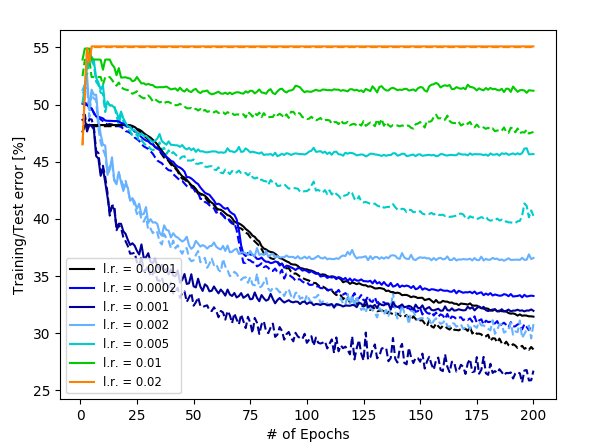
\includegraphics[scale=0.5]{DetLearnRate2DConvNN20PerceptFinal.png}
  \caption{Training error and test error for different learning rates (l.r.), exemplary shown for a 1D conventional NN with 1 hidden layer comprising of 600 perceptrons.}
  \label{fig::DeterminationLearningRate1DConvNN}
\end{figure}
\begin{figure}[H]
	\centering
  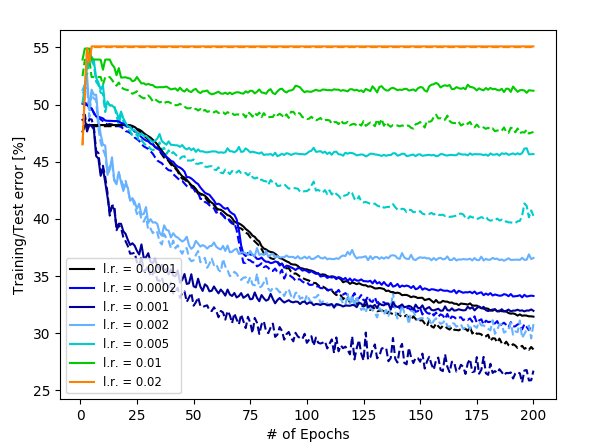
\includegraphics[scale=0.5]{DetLearnRate2DConvNN20PerceptFinal.png}
  \caption{Training error and test error for different learning rates (l.r.) exemplary shown for a 2D convolutional NN with 4 hidden layers, each comprising of 20 perceptrons.}
  \label{fig::DeterminationLearningRate2DConvNN}
\end{figure}


\subsection{Impact of weight sharing and auxiliary loss}
Fig.~\ref{fig::ImpactOfFeatures1DNN} and Fig.~\ref{fig::ImpactOfFeatures2DNN} show exemplary the training evolution of a 1D and 2D NN respectively when using weight-sharing and/or auxiliary losses. One can clearly see that weight sharing significantly improves the training time and furthermore leads to an improved accuracy of almost 10\% for the test error. The introduction of an auxiliary loss alone improves the accuracy in a similar manner, however the training time is significantly larger (200 epochs) than for the weight-sharing (50-75 epochs). For the 2D convolutional network a similar trend is visible, however longer training times are required to reach a conclusion on the obtained accuracies. 
\begin{figure}[H]
	\centering
  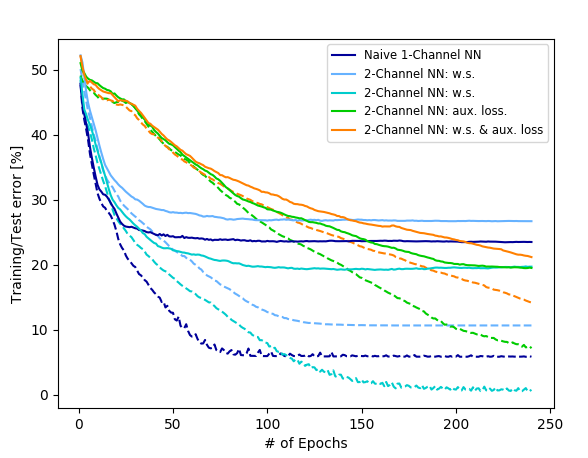
\includegraphics[scale=0.5]{ImpactOfFeatures1DNN.png}
  \caption{Training error and test error for different learning rates (l.r.), exemplary shown for a 1D conventional NN with 1 hidden layer comprising of 600 perceptrons.}
  \label{fig::ImpactOfFeatures1DNN}
\end{figure}
\begin{figure}[H]
	\centering
  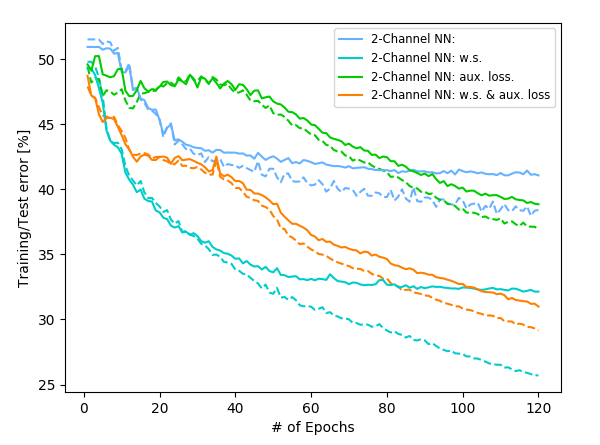
\includegraphics[scale=0.5]{ImpactOfFeatures2DNN.png}
  \caption{Training error and test error for different learning rates (l.r.), exemplary shown for a 2D conventional NN with 1 hidden layer comprising of 600 perceptrons.}
  \label{fig::ImpactOfFeatures2DNN}
\end{figure}
The results shown above have also been observed in models with the same architecture but with higher number of perceptrons per layer, in the range of [20 - 100] and [100 - 600] for the convolutional and conventional model architectures respectively. 

\section{Discussion}
Based on this work we can conclude that weight sharing improves training time and accuracy significantly.
Additional auxiliary loss, however, only slightly improves the accuracy while increases the training time significantly as compared to weight sharing only using regular loss. The combination of both of these features -- weight sharing and auxiliary loss -- does not have a strong additive effect on accuracy. These observations hold up in both cases of convolutional and non convolutional networks architectures. 
Moving forward, one could still investigate more architectures, vary the number of layers, and add new features such as batch normalization or dropout in order to verify these observations.

%\addtolength{\textheight}{-12cm}

\begin{thebibliography}{99}

\bibitem{c1} Robin Tommy, Gullapudi Sundeep and Hima Jose, 2017. Automatic Detection and Correction of Vulnerabilities using Machine Learning.
\bibitem{c2} Sanjay Kumar, Ari Viinikaineny and Timo Hamalainenz, 2016. Machine Learning Classification Model For Network Based Intrusion Detection System
\bibitem{c3} Gauri Kalnoor and Jayashree Agarkhed, 2016. Preventing Attacks and Detecting Intruder for Secured Wireless Sensor Networks.
\bibitem{c4} Hsiu-Chuan Huang, Zhi-Kai Zhang, Hao-Wen Cheng, and Shiuhpyng Winston Shieh, 2017. Web Application Security: Threats, Countermeasures, and Pitfalls


\end{thebibliography}




\end{document}
